\begin{frame}{第十六讲、函数的极值与最值}
	\linespread{1.5}
	\begin{enumerate}
	  \item {\bf 内容与要求}{\b( \S 5.1 )}
	  \begin{itemize}
% 	    \item 理解导数与函数单调性的关系
	    \item 理解极值与最值的概念
% 	    \begin{itemize}
% 	      \item 了解隐函数和参数方程的高阶导数计算方法
% 	    \end{itemize}
	    \item 熟练掌握函数极值的必要、充分条件
	    \item 了解最优化问题
	  \vspace{1em}
	  \end{itemize}
	  \item {\bf 课后练习:}
	  \begin{itemize}
	    \item 书面作业:{\b 习题5.1:5,6,7,9,12,14}
 	    \item 思考题:{\b 习题5.1:10,11,13}
	  \end{itemize}
	\end{enumerate}
\end{frame}



\begin{frame}{\bf 第五章\; 导数的应用}
	\linespread{1.2}
	\begin{enumerate}\pause 
	  \item {\bf 函数的极值与最值}
	  \begin{itemize}
	    \item {\b 给定函数及其定义区间,如何求其最大(小)值?}
	  \end{itemize}\pause 
	  \item {\bf 微分中值定理}
	  \begin{itemize}
	    \item {\b 函数值满足特定性质时,能间接得到导数的哪些性质?}
	  \end{itemize}\pause 
	  \item {\bf Taylor公式与可导函数的多项式逼近}
	  \begin{itemize}
	    \item {\b 能否用易于计算、分析的“简单”函数近似表示指定的函数?}
	  \end{itemize}\pause 
	  \item {\bf 函数的单调性、凹凸性与曲率}
	  \begin{itemize}
	    \item {\b 导数和高阶导数的性质能反映出函数曲线的哪些几何特征?}
	  \end{itemize}\pause 
	  \item {\bf L'Hospital法则}
	  \begin{itemize}
	    \item {\b 计算函数极限的“利器”}
	  \end{itemize}
	\end{enumerate}
\end{frame}

% \begin{frame}[<+->]{\bf 第五章\; 导数的应用}
% 	\linespread{1.5}
% 	\begin{enumerate}
% 	  \item {\bf 函数的极值与最值}
% 	  \begin{itemize}
% 	    \item {\b 给定函数及其定义区间,如何求其最大(小)值和最大(小)值点?}
% 	  \end{itemize}
% 	  \item {\bf 微分中值定理}
% 	  \begin{itemize}
% 	    \item {\b 函数值满足特定性质时,能间接得到导数的哪些性质?}
% 	  \end{itemize}
% 	  \item {\bf Taylor公式与可导函数的多项式逼近}
% 	  \begin{itemize}
% 	    \item {\b 能否用易于计算和分析的“简单”函数来近似表示指定的函数?}
% 	  \end{itemize}
% 	\end{enumerate}
% \end{frame}
% 
% \begin{frame}[<+->]{\bf 第五章\; 导数的应用}
% 	\linespread{1.5}
% 	\begin{enumerate}
% 	  \addtocounter{enumi}{3}
% 	  \item {\bf 函数的单调性、凹凸性与曲率}
% 	  \begin{itemize}
% 	    \item {\b 导数和高阶导数的性质能反映出函数曲线的哪些几何特征?}
% 	  \end{itemize}
% 	  \item {\bf L'Hospital法则}
% 	  \begin{itemize}
% 	    \item {\b 计算函数极限的“利器”}
% 	  \end{itemize}
% 	\end{enumerate}
% \end{frame}

% \begin{frame}{第十八讲、函数的极值与最值}
% 	\linespread{1.5}
% 	\begin{enumerate}
% 	  \item {\bf 内容与要求}{\b( \S 5.1 )}
% 	  \begin{itemize}
% % 	    \item 理解导数与函数单调性的关系
% 	    \item 理解极值与最值的概念
% % 	    \begin{itemize}
% % 	      \item 了解隐函数和参数方程的高阶导数计算方法
% % 	    \end{itemize}
% 	    \item 熟练掌握函数极值的必要、充分条件
% 	    \item 了解最优化问题
% 	  \vspace{1em}
% 	  \end{itemize}
% 	  \item {\bf 课后练习:}
% 	  \begin{itemize}
% 	    \item 书面作业:{\b 习题5.1:5,6,7,9,12,14}
%  	    \item 思考题:{\b 习题5.1:10,11,13}
% 	  \end{itemize}
% 	\end{enumerate}
% \end{frame}

% \section{导数与函数的单调性}
% 
% \begin{frame}{导数与函数的单调性}
% 	\linespread{1.2}
% 	\begin{block}{{\bf 定理5.4.1}\hfill P263}
% 		设函数$f(x)$在$[a,b]$上连续,在$(a,b)$内可导,则
% 		\begin{enumerate}
% 		  \item 若在$(a,b)$内,$f\,'(x)>0$,$f(x)$在$[a,b]$上严格单调递增;
% 		  \item 若在$(a,b)$内,$f\,'(x)<0$,$f(x)$在$[a,b]$上严格单调递减;
% 		\end{enumerate}
% 	\end{block}
% 	\begin{exampleblock}{{\bf 例1}\hfill P264-例1 }
% 		讨论函数$y=x-\sin x$与$y=e^x-x-1$的单调性。
% 	\end{exampleblock}
% \end{frame}

\begin{frame}{复习与回顾}
	\linespread{1.2}\pause 
	{\bf 连续函数在有界闭区间上的最值定理:}\\[1ex]
% 	\vspace{1ex}
	\pause 
	设$f(x)\in C[a,b]$,则\pause 
	\begin{itemize}
	  \item $f(x)$在$[a,b]$上可取到最大和最小值\pause 
	  \item 存在$m,M$,\pause 以及点$x_m,x_M\in[a,b]$,\pause 使对任意$x\in[a,b]$\pause 
	  $$m=f(x_m)\leq f(x)\leq f(x_M)=M$$
	\end{itemize}
	\pause 
	{\ba{ 问题:}}{\b 如何求得以上的$m,M$和$x_m,x_M$?}
\end{frame}

\begin{frame}
	\linespread{1.2}
	\begin{exampleblock}{{\bf 例1}\hfill P224-例1 }
		画出函数$f(x)=3x^4-4x^3-12x^2+3$在区间$[-2,3]$,通过
		观察求其最大和最小值。
	\end{exampleblock}
	\begin{columns}
		\column{.7\textwidth}
		\begin{center}
			\only<1-2>{\uncover<2>{
			\begin{center}\resizebox{!}{5cm}{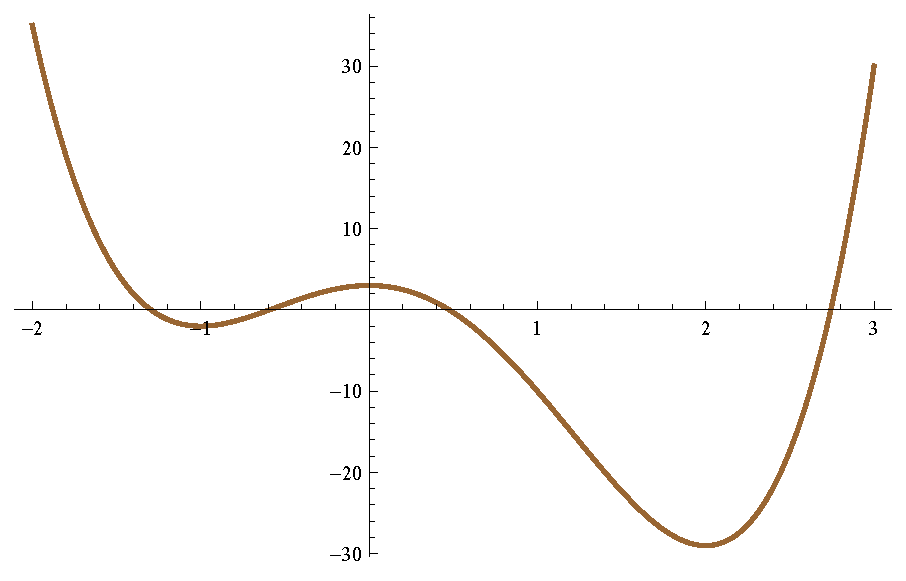
\includegraphics{./images/ch5/fmm_ori.pdf}}
			\end{center}}}
			\only<3-6>{\resizebox{!}{5cm}{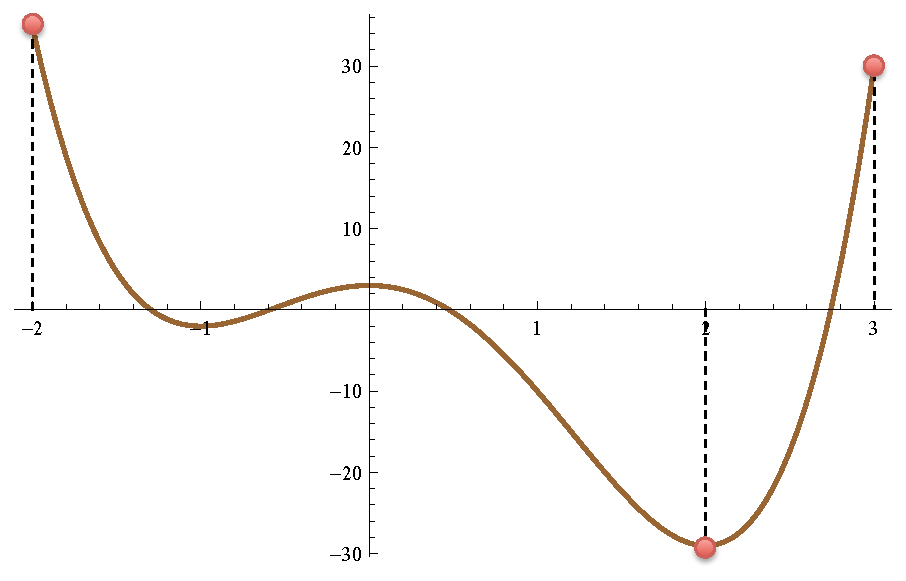
\includegraphics{./images/ch5/fmm_mark.pdf}}}
 			\only<7->{\resizebox{!}{5cm}{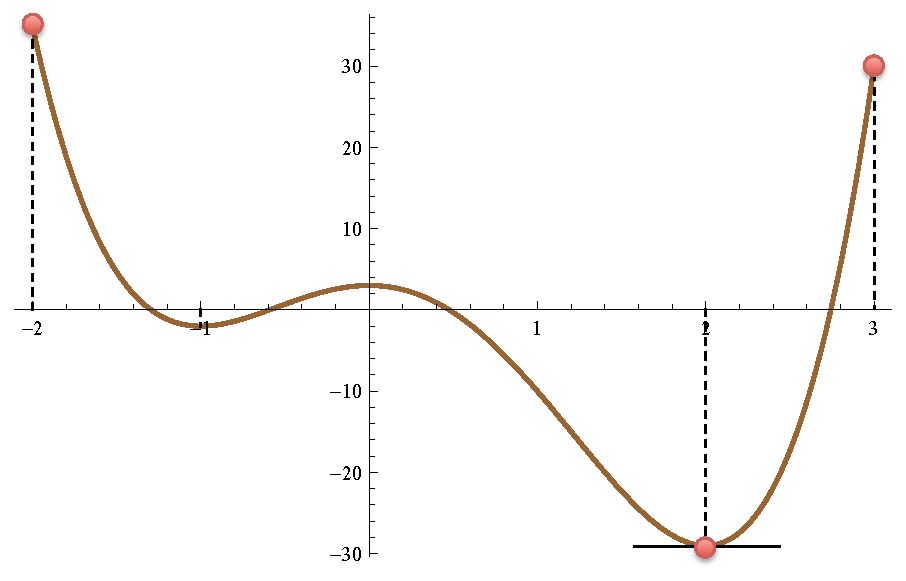
\includegraphics{./images/ch5/fmm_bar.pdf}}}
		\end{center}
		\column{.3\textwidth}
		\onslide<4->
			$f(-2)=35$\\[1em]
		\onslide<5->
			$f(3)=30$\\[1em]
		\onslide<6->
			$f(2)=-29$
	\end{columns}
\end{frame}

\begin{frame}{Fermat引理}
	\linespread{1.2}\pause 
	\begin{block}{{\bf 定理5.1.1}\hfill P226}
		若函数$f(x)$在$x_0$处可导,且在$x_0$的某邻域内,有
		$$f(x)\geq f(x_0)\quad (\mbox{或}\quad f(x)\leq f(x_0))$$
		则$f\,'(x_0)=0$。
	\end{block}\pause 
% 	\begin{exampleblock}{{\bf 例1}\hfill P224-例1 }
% 		求函数$f(x)=3x^4-4x^3-12x^2+3$在区间$[-2,3]$上的最大和最小值。
% 	\end{exampleblock}
	\begin{columns}
		\column{.25\textwidth}
		\begin{center}
			\resizebox{!}{3cm}{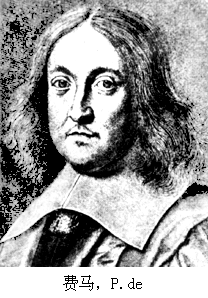
\includegraphics{./images/ch5/Fermat.png}}
		\end{center}\pause 
		\column{.75\textwidth}
			\begin{itemize}
			  \item {\ba{ the prince of amateurs}}\pause 
			  \item \alert{{\bf Fermat大定理:}}$n>2$时,方程$x^n+y^n=z^n$没有整数解
			\end{itemize}
	\end{columns}
\end{frame}

\begin{frame}
	\linespread{1.2}
	\begin{exampleblock}{{\bf 例1}\hfill P224-例1 }
		求函数$f(x)=3x^4-4x^3-12x^2+3$在区间$[-2,3]$上的最大和最小值。
	\end{exampleblock}\pause 
% 	\begin{columns}
% 		\column{.6\textwidth}
			\begin{center}
				\resizebox{!}{6cm}{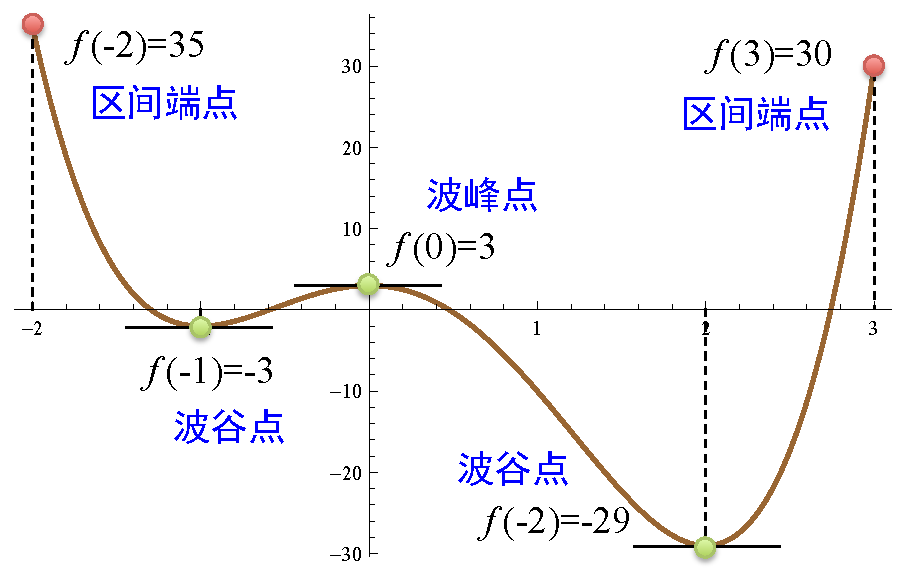
\includegraphics{./images/ch5/fmm_pt.pdf}}
			\end{center}
% 		\column{.4\textwidth}
% 	\end{columns}
% 	\begin{center}
% 	  {\bb 波峰点、波谷点$\Longrightarrow$极值点}
% 	\end{center}
\end{frame}

\begin{frame}{极值的概念}
	\linespread{1.2}\pause 
	\begin{block}{{\bf 定义5.1.1}\hfill P225}
		设在$x_0$的某去心邻域内,恒有
		$$f(x)<f(x_0)\quad (\mbox{或}\quad f(x)>f(x_0)),$$
		则称$f(x_0)$是$f(x)$的一个{\bb 极大(小)值},$x_0$称为$f(x)$的一个{\bb 极值点}。
	\end{block}\pause 
	\alert{
	\begin{itemize}
	  \item 函数在极值点处未必可导\pause 
	  \item 可导函数极值点处的导数为零\pause 
	  \item 导数为零的点({\bb 驻点})未必是极值点
	\end{itemize}}
\end{frame}

\begin{frame}{极值判定的充分条件}
	\linespread{1.2}\pause 
	\begin{block}{{\bf 定理5.1.2}\hfill P227}
		设$f(x)$在$x_0$附近连续,若$f(x)$在$x_0$两侧单调性发生改变,
		则$f(x)$在$x_0$取极值。
	\end{block}\pause 
	{\bf 注:}连续函数单调性的分界点是函数的极值点。\pause 
	\begin{center}
		\resizebox{!}{4cm}{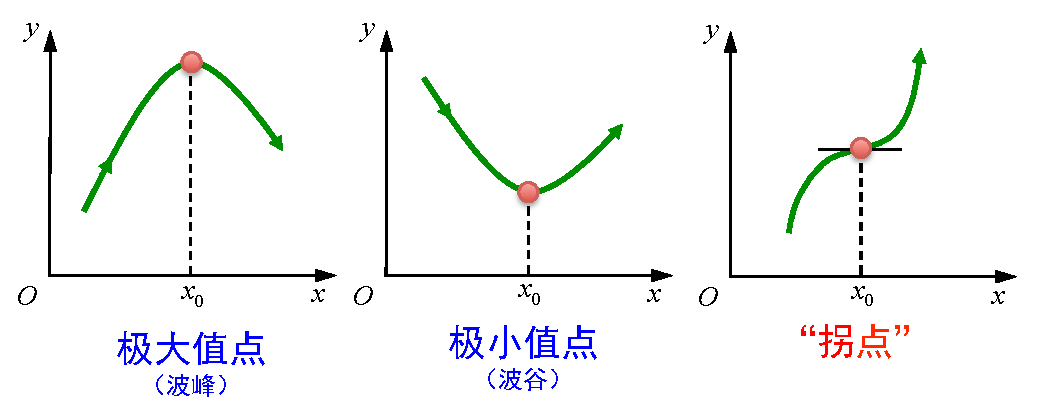
\includegraphics{./images/ch5/edge_pt.pdf}}
	\end{center}
\end{frame}

\begin{frame}{极值与最值的关系}
	\linespread{1.2}\pause 
	\begin{exampleblock}{{\bf 例2:}判断以下说法的正误\hfill }\pause 
		\begin{enumerate}
		  \item 函数的极大值一定是最大值\quad\pause  (\alert{$\times$})\pause 
		  \item 函数的最大值一定是极大值\quad\pause  (\alert{$\times$})\pause 
		  \item 函数的极大值一定比极小值大\quad\pause  (\alert{$\times$})\pause 
		\end{enumerate}
	\end{exampleblock}
	{\ba{思考:}}{\b 在闭区间上,函数可能在什么位置取到最值?}\pause 
	\vspace{-1em}
	\begin{columns}
		\column{.33\textwidth}
			\begin{center}
				\resizebox{.99\textwidth}{3.5cm}{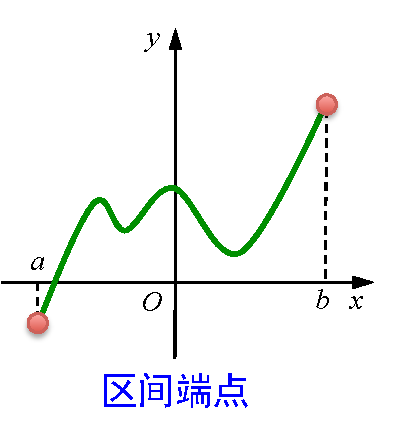
\includegraphics{./images/ch5/mm1.pdf}}\pause
							\end{center}
		\column{.33\textwidth}
			\begin{center}
				\resizebox{.99\textwidth}{3.5cm}{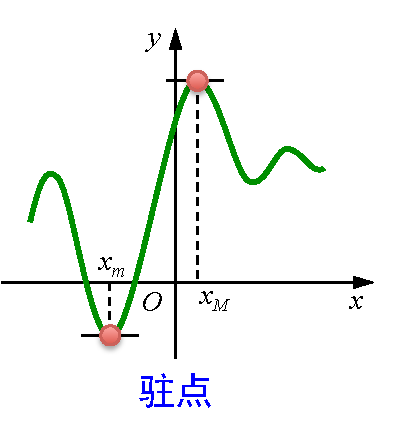
\includegraphics{./images/ch5/mm2.pdf}}\pause
							\end{center}
		\column{.33\textwidth}
			\begin{center}
				\resizebox{.99\textwidth}{3.5cm}{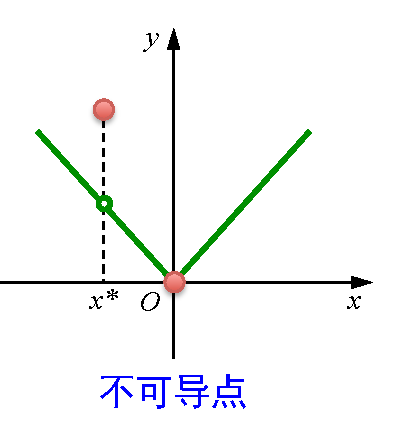
\includegraphics{./images/ch5/mm3.pdf}}
			\end{center}
	\end{columns}
\end{frame}

\begin{frame}{求闭区间上连续函数的最值}
	\linespread{1.2}\pause 
	{\ba{ 步骤:}}\pause 
	\begin{enumerate}
	  \item 确定函数在区间内的所有{\b 驻点}和{\b 不可导点} \,$x_1,x_2,$ $\ldots,x_n$\pause 
	  \item 逐个计算
	  $f(a),f(x_1),f(x_2),\ldots,f(x_n),f(b)$,
	  {\b 比较求得最大和最小值}。\pause 
	\end{enumerate}
	\begin{exampleblock}{{\bf 例3}\hfill P228-例3}
		求$f(x)=|x|e^x$在区间$[-2,1]$上的最大和最小值。
	\end{exampleblock}\pause 
	{\ba{ 思考:}}如何求函数在开区间上的最值?
\end{frame}

\begin{frame}{最优化问题简介}
	\linespread{1.2}\pause 
% 	{\bf 最优化问题:}在“资源”有限的条件上,实现特定目标的最大(小)化?
% 	{\bf 举例:}
	\begin{itemize}
	  \item 给定边长,求所能围成的矩形区域的最大面积?\pause 
	  \item 给定原材料,生产各种商品所能获得最大利润?\pause 
	  \item 为达到特定生产收益,所需投入的最少资源?\pause 
	  \item \ldots \ldots\pause 
	\end{itemize}
	\begin{alertblock}{{\bf 最优化问题}\hfill }\pause 
		\begin{description}
		\item[{\ba{ 目标:}}] \pause 求函数$f(x)$的最大(小)值以及对应的最大(小)值点\pause 
		\item[{\ba{ 约束:}}] \pause 变量$x$满足一定的条件,\pause 例如:$x\in[a,b]$
		\end{description}
	\end{alertblock}
\end{frame}

\begin{frame}
	\linespread{1.2}
	\begin{exampleblock}{{\bf 例4}\hfill P230-例5}
		一个边长为$a$的方形铁皮,在四角各剪去一个边长为$x$的小正方形,然后折成
		一个无盖的长方体容器,问当$x$取何值时,长方体容器的容积最大?
	\end{exampleblock}\pause 
	\begin{center}
		\resizebox{!}{5cm}{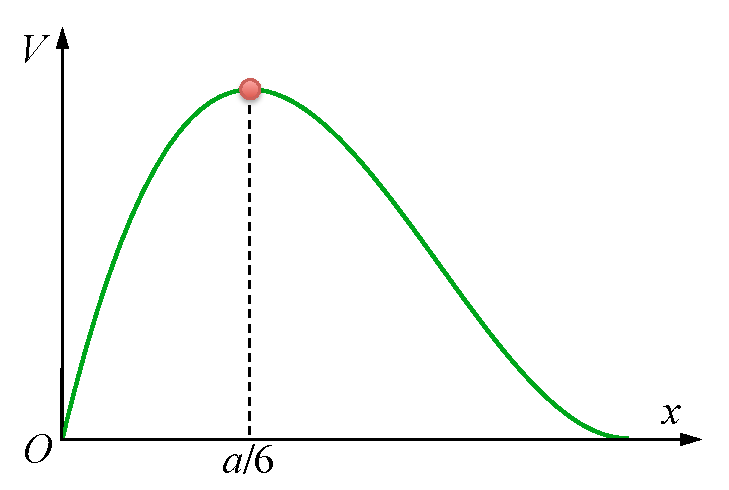
\includegraphics{./images/ch5/box.pdf}}
	\end{center}
\end{frame}

\begin{frame}
	\linespread{1.2}
	\begin{exampleblock}{{\bf 例5}\hfill P230-例4}
		用输油管连接离海岸12km的钻井平台和沿岸往下20km处的炼油厂。已知水下和陆上铺设
		管道的成本分别是每公里50万元和30万元,问该如何设计线路,使总的建设成本最低?
	\end{exampleblock}\pause 
	{\ba{解题过程:}}\pause 
	\begin{enumerate}
	  \item {\b 理解题意:}画图、定义变量\pause 
	  \item {\b 建立关系:}目标函数表达式\pause 
	  \item {\b 求解最值}
	\end{enumerate}
\end{frame}

%=====================================

\begin{frame}[<+->]{小结}
	\linespread{1.2}
 	{\ba{问题:}}{\b 如何求闭区间上函数的最值和最值点?}\bigskip\pause
	\begin{enumerate}
	  \item {\bf 极值的概念}
	  \begin{itemize}
	    \item 极值和最值的区别
	    \item 可导函数极值的必要条件
	  \end{itemize}
	  \item {\bf 闭区间上函数的最值点}
	  \begin{itemize}
	    \item 驻点
	    \item 不可导点
	    \item 区间端点
	  \end{itemize}
	  \item {\bf 最优化问题}
	\end{enumerate}
% 	\bigskip
% 	\pause
% 	\centerline{\ba{请自行阅读第六章\S 6.3节}}
\end{frame}